% UHK FIM Beamer Template

\documentclass[aspectratio=169]{beamer}
% \documentclass[aspectratio=43]{beamer}

\usepackage[czech]{babel}

\usepackage{graphicx} % Pro vkládání obrázků
% \usepackage[absolute,overlay]{textpos} % Pro přesné umístění prvků

\usepackage{lmodern}          % Moderní font s podporou češtiny
\usepackage[utf8]{inputenc}   % Kódování UTF-8
\usepackage[T1]{fontenc}      % Fontová encodace pro české znaky
\usepackage{tikz}
\usetikzlibrary{calc}

\usepackage{csquotes}
\usepackage{xcolor}
\usepackage{pgfplots}
\usepackage{booktabs} % Pro profesionální tabulky s \toprule, \midrule, \bottomrule
\usepackage{multirow} % Pro slučování řádků v tabulkách
\usepackage{pgfgantt}
\usepackage{animate}
\usepackage{xmpmulti}
\usepackage{subcaption} % Pro pod-obrázky
\usepackage{adjustbox} % Pro snadné přizpůsobení velikosti
\usepackage{tabularx} % Přidejte do preambule
\usepackage{pgfplots}
\usepackage{pgfplotstable}
\pgfplotsset{compat=1.18}

\usepgfplotslibrary{polar}

\usepackage[
backend=biber,
style=ext-authoryear,
citestyle=numeric, giveninits=false, maxnames=1, uniquename=false
]{biblatex}
\addbibresource{references.bib}

\renewcommand*{\bibfont}{\scriptsize}

% Přepíšeme formát citace
\renewbibmacro*{cite:author}{%
  \ifnameundef{author}{% Pokud není definován autor
    \printfield{title}% Použije pole "title"
  }{%
    \printnames[given-family]{author}% Zobrazí prvního autora
    \ifnumgreater{\value{listtotal}}{1}{\addspace\bibstring{andothers}}{}%
  }%
  \setunit{\addspace}%
  \printtext[parens]{\printfield{year}}% Rok v závorce
}

% Makro pro \textcite
\DeclareCiteCommand{\textcite}{%
  \scriptsize
  \usebibmacro{cite:author}%
  \setunit{\addspace}%
  \printtext[bibhyperref]{[\printfield{labelnumber}]}
}{%
}{%
}{%
}

% \usepackage{helvet}
% \renewcommand{\familydefault}{\sfdefault}

% Define color scheme based on extracted colors
\definecolor{uhkDark1}{RGB}{0,0,0} % Placeholder for dk1
\definecolor{uhkLight1}{RGB}{255,255,255} % Placeholder for lt1
\definecolor{uhkAccent1}{RGB}{0,159,224} % Placeholder for accent1
\definecolor{uhkAccent2}{RGB}{0,176,80} % Placeholder for accent2
\definecolor{uhkAccent3}{RGB}{255,192,0} % Placeholder for accent3
\definecolor{uhkAccent4}{RGB}{192,80,77} % Placeholder for accent4
\definecolor{uhkAccent5}{RGB}{155,187,89} % Placeholder for accent5
\definecolor{uhkAccent6}{RGB}{79,129,189} % Placeholder for accent6

\definecolor{customblue}{RGB}{0,159,224}

% Hide navigation symbols
% \setbeamertemplate{navigation symbols}{}

% Increase padding for slides
% \addtobeamertemplate{frametitle}{}{
%     \vspace{1cm}
% }

\setbeamertemplate{frametitle}{
    \vspace{0.7cm} % Add space above the title
    \nointerlineskip
    % \hspace*{0.5cm} % Add space to the left of the title
    \insertframetitle\par
    \vspace{0.3cm} % Add space below the title
}
% \setbeamersize{text margin left=1cm,text margin right=1.5cm}

% Set theme colors
\setbeamercolor{palette primary}{fg=uhkLight1,bg=uhkDark1}
\setbeamercolor{palette secondary}{fg=uhkDark1,bg=uhkAccent1}
\setbeamercolor{palette tertiary}{fg=uhkLight1,bg=uhkAccent2}

% Fonts
\setbeamerfont{title}{family=\sffamily,series=\bfseries,size=\LARGE}
\setbeamerfont{frametitle}{family=\sffamily,series=\bfseries,size=\Large}
\setbeamerfont{normal text}{family=\sffamily}

% Title page setup
\title[Short Title]{Využití umělé inteligence v oblasti\\reprodukční medicíny}
\author{Michal Dobrovolný}
\institute[UHK FIM]{University of Hradec Kralove, Faculty of Informatics and Management}
\date{\today}

\setbeamertemplate{title page}{
    % Logo vlevo nahoře
    \begin{tikzpicture}[remember picture,overlay]
        \node[anchor=north west] at ([xshift=0.5cm,yshift=-0.5cm]current page.north west) {
            
\includegraphics[width=6cm]{img/logo-placeholder2.png} % Změňte "logo.png" na cestu k vašemu logu
        };
    \end{tikzpicture}
    
    % Obrázek vpravo od 2/3 stránky
    \begin{tikzpicture}[remember picture,overlay]
        \node[anchor=north east] at ([xshift=-0.5cm,yshift=0.13cm]current page.north east) {
            
\includegraphics[height=8cm]{img/devider2.png} % Změňte "image.png" na cestu k obrázku
        };
    \end{tikzpicture}

    % Text (title a author) zarovnaný vlevo od obrázku
    \begin{center}
        \vspace{1cm} % Posunutí dolů
        \hspace*{-2.5cm} % Posunutí doleva pro zarovnání k obrázku
        \begin{minipage}[t]{0.8\textwidth} % Šířka textového bloku
            \raggedleft
            {\Large \textbf{\textcolor{uhkAccent1}{\inserttitle}}} \\[0.1cm]
            {\large \insertauthor}
        \end{minipage}
    \end{center}
}



\setbeamertemplate{frametitle}{
    \begin{tikzpicture}[remember picture,overlay]
        % Logo vlevo nahoře
        \node[anchor=north west] at ([xshift=0.5cm,yshift=0.17cm]current page.north west) {
            
\includegraphics[height=2cm]{img/logo-placeholder.png} % Změňte na cestu k vašemu logu
        };

        \fill[customblue] 
            ([xshift=5.5cm, yshift=-0.5cm]current page.north west) -- % Horní hrana obdélníku
            ([xshift=5.35cm, yshift=-0.65cm]current page.north west) -- % 45° dolů vlevo
            ([xshift=5.35cm, yshift=-0.85cm]current page.north west) -- % Rovně dolů
            ([xshift=5.2cm, yshift=-1cm]current page.north west) -- % 45° dolů vlevo
            ([xshift=5.35cm, yshift=-1.15cm]current page.north west) -- % Rovně dolů
            ([xshift=5.35cm, yshift=-1.35cm]current page.north west) -- % 45° dolů vpravo
            ([xshift=5.5cm, yshift=-1.5cm]current page.north west) -- % Dolní hrana obdélníku
            ([xshift=0cm, yshift=-1.5cm]current page.north east) -- % Pravý dolní roh obdélníku
            ([xshift=0cm, yshift=-0.5cm]current page.north east) -- % Pravý horní roh obdélníku
            cycle;
        
        % Název snímku (zarovnaný doprava, bílá barva)
        \node[anchor=east, text=white, font=\large\bfseries] at ([xshift=-0.1cm,yshift=-1cm]current page.north east) {
            \insertframetitle
        };
    \end{tikzpicture}
    \vspace*{1.5cm}
}

\begin{document}

% Title page
\begin{frame}
    \titlepage
\end{frame}










\section{Proč se problematikou zabývat}



\begin{frame}{Důvody mužské neplodnosti dle WHO}
    \begin{columns}
        \column{0.5\textwidth}
        \begin{itemize}
            \item \textbf{Životní styl:}
            \begin{itemize}
                \item Kouření tabáku
                \item Nadměrná konzumace alkoholu
                \item Užívání rekreačních drog
                \item Nezdravé stravovací návyky a nedostatek fyzické aktivity
                \item Chronický stres
            \end{itemize}
        \end{itemize}
        
        \column{0.5\textwidth}
        \begin{itemize}
            \item \textbf{Environmentální faktory:}
            \begin{itemize}
                \item Expozice toxickým látkám (např. pesticidům, těžkým kovům)
                \item Dlouhodobé působení vysokých teplot
            \end{itemize}
            \item \textbf{Zdravotní faktory:}
            \begin{itemize}
                \item Obezita a hormonální nerovnováha
                \item Infekce nebo záněty
            \end{itemize}
            \item \textbf{Stárnutí:}
            \begin{itemize}
                \item Pokles kvality spermií s věkem
                \item Zhoršení genetické integrity spermií
            \end{itemize}
        \end{itemize}
    \end{columns}
    \centering
    \scriptsize
    Zdroj WHO \textcite{world_health_organization_who_2021}
\end{frame}

\begin{frame}{Mikroskopická analýza}    
    \begin{columns}
        \column{0.5\textwidth}
        \begin{itemize}
            \item \textbf{Počet spermií:}
            \begin{itemize}
                \only<1>{\item Počítání spermií.}
                \only<2>{\item \textcolor{uhkAccent1}{Počítání spermií.}}
            \end{itemize}
        
            \item \textbf{Pohyblivost (motilita):}
            \begin{itemize}
                \item Kategorizace spermií na:
                \begin{itemize}
                    \item Progresivně pohyblivé,
                    \item Neprogresivně pohyblivé,
                    \item Nepohyblivé.
                \end{itemize}
            \end{itemize}
        \end{itemize}
        
        \column{0.5\textwidth}
        \begin{itemize}
            \item \textbf{Morfologie:}
            \begin{itemize}
                \item Barvení spermií (např. Papanicolaou metoda).
                \only<1>{\item Klasifikace podle normálních a abnormálních tvarů (hlavička, střední část, bičík).}
                \only<2>{\item \textcolor{uhkAccent1}{Klasifikace podle normálních a abnormálních tvarů (hlavička, střední část, bičík).}}
            \end{itemize}
        
            \item \textbf{Vitalita:}
            \begin{itemize}
                \item Použití barvicích metod (např. eosin-nigrosin test).
                \item Identifikace živých a mrtvých spermií.
            \end{itemize}
        \end{itemize}
    \end{columns}
\end{frame}


\begin{frame}{Proč se tématem zabývat}
    \begin{figure}
	\begin{tikzpicture}[scale=.8]
		\begin{axis}[
			ybar interval=0.8,
			%   xtick=,% reset from ybar interval
			x tick label style={/pgf/number format/1000 sep=},
			y tick label style={/pgf/number format/1000 sep=},
			height=6cm,
			width=\textwidth,
			xmin=2011,xmax=2024,
            ymajorgrids=true, % Zobrazení hlavní mřížky na ose y
            grid style=dashed % Styl mřížky (čárkovaná)
			]
			\addplot coordinates {
				(2024, 6)
				(2023, 16)
				(2022, 20)
				(2021, 16)
				(2020, 10)
				(2019, 14)
				(2018, 6)
				(2017, 8)
				(2016, 7)
				(2015, 9)
				(2014, 7)
				(2013, 5)
				(2012, 3)
				(2011, 3)
			};
			% \legend{Year}
		\end{axis}
	\end{tikzpicture}
	\caption{Roční počet publikací v databázi Web of Science. K 13.9.2024 [autor]}
	\label{publications}
	\end{figure}
    
    \centering
    \tiny Vyhledaný dotaz bez dalších filtru typů publikací \\
    (ALL = (sperm detection) AND (ALL = (computer) OR ALL=(vision)) NOT ALL = (gene) NOT ALL = (DNA))
\end{frame}








\section{Cíle}

\begin{frame}{Cíle disertační práce}
\begin{itemize}
    \item \textbf{Vytvoření datové sady:}
    \begin{itemize}
        \item Vytvoření unikátní datové sady mikroskopických obrazů, zahrnující vzorky od pacientů s nízkou koncentrací spermií.
        \item Zaměření na anotaci zdravých spermií s důrazem na jejich morfologické charakteristiky.
        \item Integrace vzorků různých pacientů s cílem zajistit dostatečnou variabilitu dat pro robustní analýzu.
    \end{itemize}
    \item \textbf{Návrh detekčního algoritmu:}
    \begin{itemize}
        \item Návrh detekčního algoritmu založeného na modelech YOLO a DINO.
        \item Optimalizace algoritmu s důrazem na vyvážení mezi vysokou přesností detekce a rychlostí analýzy.
        \item Cílem je minimalizace falešně pozitivních detekcí.
    \end{itemize}
\end{itemize}
\end{frame}


\begin{frame}{Datová sada}
    \begin{columns}
        % Left column: Human vs animal sperm
        \column{0.5\textwidth}
        \textbf{Lidská vs zvířecí spermie:}
        \begin{itemize}
            \item Lidská spermie:
            \begin{itemize}
                \item Oválná hlava.
                \item Krátký bičík.
                \item Menší velikost ve srovnání s některými zvířecími spermiemi.
            \end{itemize}
            \item Zvířecí spermie:
            \begin{itemize}
                \item Variabilní tvary (např. spirálová u ptáků, dlouhá u savců jako myši).
                \item Dlouhé bičíky umožňující rychlejší pohyb.
            \end{itemize}
        \end{itemize}

        % Right column: Healthy vs defective sperm
        \column{0.5\textwidth}
        \textbf{Zdravá vs defektní spermie:}
        \begin{itemize}
            \item Zdravá spermie:
            \begin{itemize}
                \item Symetrická hlava oválného tvaru.
                \item Přímý bičík umožňující efektivní pohyb.
            \end{itemize}
            \item Defektní spermie:
            \begin{itemize}
                \item Deformovaná hlava (např. dvojhlavá).
                \item Vakuoly nebo jiné abnormality v hlavě.
                \item Zakřivený nebo zlomený bičík.
            \end{itemize}
        \end{itemize}
    \end{columns}
\end{frame}


\begin{frame}
    \frametitle{SVIA dataset}

    \begin{figure}
        \centering
        \begin{adjustbox}{max width=0.8\textwidth}
            \begin{minipage}{0.6\textwidth}
                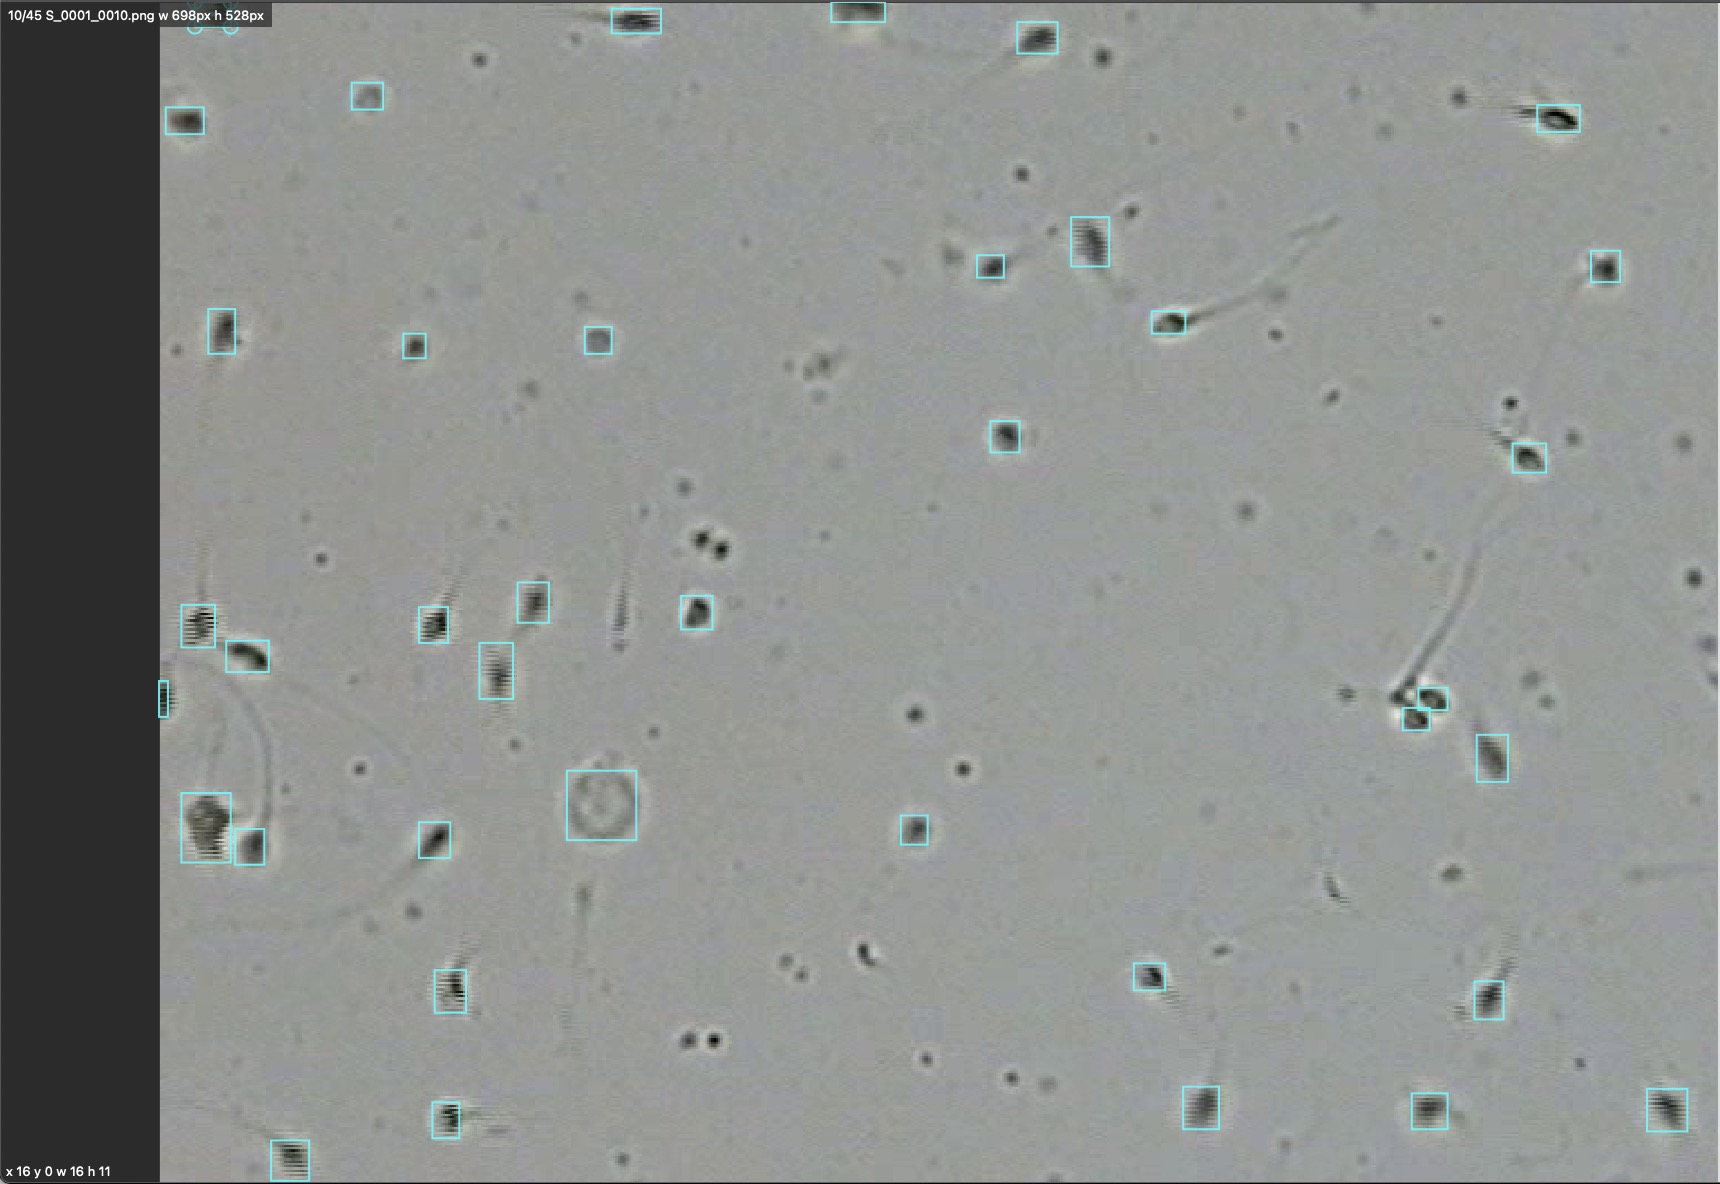
\includegraphics[width=\linewidth]{img/svia-1.jpg} % Velký obrázek vlevo
            \end{minipage}%
            \begin{minipage}{0.4\textwidth}
                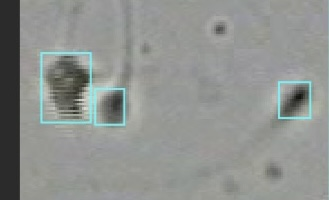
\includegraphics[width=\linewidth]{img/svia-2.jpg}\\ % První malý obrázek vpravo nahoře
                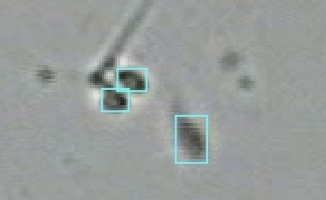
\includegraphics[width=\linewidth]{img/svia-3.jpg}  % Druhý malý obrázek vpravo dole
            \end{minipage}
        \end{adjustbox}
        \caption{Sperm Videos and Images Analysis (SVIA). \textcite{chen_svia_2022}}
        \label{fig:example}
    \end{figure}
    
\end{frame}







\section{Dataset}




\begin{frame}{Porovnání datasetů}

    \begin{table}
        \centering
        \scriptsize
        \caption{Porovnání datasetů [autor]}
        \begin{tabularx}{\textwidth}{|X||X||X|X|X|}
            \hline
            \textbf{Parametr}         & \textbf{Nový dataset}               & \textbf{SVIA \cite{chen_svia_2022}}                      & \textbf{MHSMA \cite{javadi_novel_2019}}                      & \textbf{VISEM \cite{haugen_visem_2019}}                     \\ \hline
            \textbf{Forma anotace}    & Bounding boxy                      & Bounding boxy a morfologické rysy   & Segmentace a podrobná anotace        & Metadata (počet, pohyblivost)        \\ \hline
            \textbf{Zdravé spermie}   & Ano, pouze zdravé                  & Ano, obsahuje i defektní            & Ano, obsahuje i abnormality          & Neobsahuje klasifikační metadata spermií \\ \hline
            \textbf{Defektní spermie} & Ne                                 & Ano, různé druhy defektů            & Ano, abnormality (vakuoly, hlavičky, akrozomy) & Neobsahuje klasifikační metadata spermií \\ \hline
            \textbf{Variabilita dat}  & Variabilní prostředí               & Jednotné pozadí                     & Jednotné pozadí                      & Variabilní prostředí                 \\ \hline
            \textbf{Cíl datasetu}     & Detekce zdravých spermií           & Detekce objektů                     & Klasifikace, segmentace               & Analýza pohyblivosti         \\ \hline
        \end{tabularx}
    \end{table}

\end{frame}











\section{Metodologie}

\begin{frame}{Metodologie}

    \begin{columns}
        \column{0.65\textwidth}
        \textbf{Evaluační metriky:}
        \begin{itemize}
            \item FN, FP, senzitivita, přesnost.
            \item „Intersection over Union“ (IoU), jako metrika kvality lokalizace.
            \item Mean Average Precision (mAP) pro celkové hodnocení detekčního algoritmu.
        \end{itemize}
    
        \column{0.35\textwidth}
        \begin{figure}
            \resizebox{!}{0.35\paperheight}{
            \centering
            \begin{tikzpicture}
                % Ground Truth Box
                \draw[thick, green] (0, 0) rectangle (4, 4);
                \node[align=center, green] at (-0.5, 4.5) {Ground\\Truth};
        
                % Predicted Box
                \draw[thick, blue] (2, 2) rectangle (6, 6);
                \node[align=center, blue] at (6.5, 6.5) {Prediction};
        
                % Intersection Area
                \fill[purple, opacity=0.5] (2, 2) rectangle (4, 4);
                \node[align=center, white] at (3, 3) {Intersection};
        
                % Union Annotation
                \node[align=center] at (3, -0.5) {Union};
        
                % Labels
                \node[below] at (2, 0) {X-axis};
                \node[rotate=90, above] at (0, 2) {Y-axis};
            \end{tikzpicture}
            }
            \caption{Metrika kvality lokalizace. [autor]}
        \end{figure}
    \end{columns}
\end{frame}


% Frame s diagramem
\begin{frame}{Metodologie}

    \begin{columns}
        % Left column: Human vs animal sperm
        \column{0.4\textwidth}
    \textbf{Architektura algoritmu:}
    \begin{itemize}
        \item Detekční algoritmus založený na YOLOv5 a DINOv2 pro zvýšení přesnosti.
        \item Použití prahové hodnoty správnosti detekce 0,3.
    \end{itemize}
    
        \column{0.6\textwidth}
    \begin{figure}
        \centering
        \resizebox{1.1\textwidth}{!}{
            \begin{tikzpicture}[node distance=2.5cm, scale=0.9, transform shape]
            
            % Styly uzlů a šipek
            \tikzstyle{startstop} = [rectangle, rounded corners, minimum width=2.5cm, minimum height=1cm, text centered, draw=black, fill=red!20]
            \tikzstyle{process} = [rectangle, minimum width=2.5cm, minimum height=1cm, text centered, draw=black, fill=blue!20]
            \tikzstyle{data} = [trapezium, trapezium left angle=70, trapezium right angle=110, minimum width=2.5cm, minimum height=1cm, text centered, draw=black, fill=orange!30]
            \tikzstyle{arrow} = [thick,->,>=stealth]
            
            % Uzly diagramu
            \node (input) [startstop] {Vstup: Mikroskopický obraz};
            \node (yolo) [process, below of=input] {Detekce spermií pomocí YOLO};
            \node (boundingbox) [data, below of=yolo] {Výstup: Bounding boxy};
            \node (dino) [process, right of=boundingbox, xshift=4cm] {Klasifikace pomocí DINO};
            \node (output) [startstop, below of=dino] {Výstup: Zdravé spermie};
            
            % Šipky propojující uzly
            \draw [arrow] (input) -- (yolo);
            \draw [arrow] (yolo) -- (boundingbox);
            \draw [arrow] (boundingbox.east) -- (dino.west);
            \draw [arrow] (dino) -- (output);
            
            % Popisky po stranách
            \node at (-4, -1.5) [text width=4cm] {\textbf{YOLO:} Rychlá detekce spermií};
            \node at (9, -3.5) [text width=5cm] {\textbf{DINO:} Klasifikace spermií};
            
            \end{tikzpicture}
        }
        \caption{Diagram detektoru. [autor]}
    \end{figure}
    \end{columns}
\end{frame}









\section{Výsledky}

\begin{frame}{Dosažené výsledky detekce}
    \centering

    \footnotesize Shrnutí modelů a jejich výsledků. \cite{rojas_sperm-cell_2022}
    \vspace{0.4cm}
    
    % Resize both tables to fit the slide
    \resizebox{\textwidth}{!}{%
        \begin{tabular}{ccccccc}
            \toprule
            \textbf{Tabulka} & \textbf{Model} & \textbf{Nano} & \textbf{Small} & \textbf{Medium} & \textbf{Large} & \textbf{Xtra} \\
            \midrule
            \multirow{4}{*}{Velikost} 
            & Velikost vstupu & \multicolumn{5}{c}{640 $\times$ 480} \\
            & Počet vrstev & 270 & 270 & 369 & 468 & 567 \\
            & Počet parametrů & 1 765k & 7 022k & 20 871k & 46 138k & 86 218k \\
            & Velikost v paměti (GB) & 0,93 & 1,73 & 3,2 & 4,97 & 7,34 \\
            \midrule
            \multirow{3}{*}{Výsledky}
            & Přesnost (\%) & 64,7 & 61,6 & 71,7 & 88,6 & 64,6 \\
            & Pokrytí (\%) & 61,4 & 64,9 & 57,8 & 52,6 & 71,9 \\
            & mAP (\%) & 69,6 & 64,6 & 66,4 & 72,1 & 68,6 \\
            \bottomrule
        \end{tabular}%
    }
\end{frame}


\begin{frame}{Dosažené výsledky detekce}

\begin{tikzpicture}
    \begin{axis}[
        ybar,
        bar width=0.5cm,
        width=.88\textwidth,
        height=0.45\textwidth,
        ymin=0, ymax=95,
        xlabel={Model},
        % ylabel={},
        symbolic x coords={Nano, Small, Medium, Large, Xtra},
        xtick=data,
        nodes near coords,
        nodes near coords align={vertical},
        every node near coord/.append style={font=\small},
        legend style={at={(-0.2,.5)}, anchor=north, font=\scriptsize},
        grid=both
    ]
        % Data for mAP
        \addplot coordinates {(Nano, 69.6) (Small, 64.6) (Medium, 66.4) (Large, 72.1) (Xtra, 68.6)};
        
        % Optional: Data for other attributes like precision or parameter size
        % Uncomment if needed
        \addplot coordinates {(Nano, 64.7) (Small, 61.6) (Medium, 71.7) (Large, 88.6) (Xtra, 64.6)}; % Precision
        \addplot coordinates {(Nano, 1.765) (Small, 7.022) (Medium, 20.871) (Large, 46.138) (Xtra, 86.218)}; % Parameters (scaled)
        
        \legend{mAP (\%), přesnost (\%), parametrů (M)}
    \end{axis}
\end{tikzpicture}
\end{frame}


\section{Další směrování práce}


\begin{frame}{Další směrování práce}
        % \vspace*{-1cm} % Posun nahoru
    \begin{figure}[ht]
        \centering
        \hspace*{-1cm} % Posun doleva
        \begin{ganttchart}[
            hgrid,
            vgrid,
            bar label font=\tiny, % Zmenšení fontu popisků
            title label font=\scriptsize, % Zmenšení fontu nadpisů
            group label font=\scriptsize, % Zmenšení fontu skupin
            milestone label font=\tiny, % Zmenšení fontu milníků
            x unit=0.42cm, % Zmenšení šířky jednotky
            y unit title=0.5cm, % Zmenšení výšky nadpisů
            y unit chart=0.4cm, % Zmenšení výšky pruhů
            progress label text={}, % Skrytí štítků pro průběh
            bar height=0.3 % Zmenšení výšky pruhů
        ]{1}{18}
        
          \gantttitle{2021}{4} \gantttitle{2022}{4} \gantttitle{2023}{4} \
          \gantttitle{2024}{4} \gantttitle{2025}{2} \\
          
          \ganttgroup[progress=100]{Detekce spermií pomocí YOLO}{1}{10} \\
          \ganttbar[progress=100]{Příprava datové sady}{1}{8} \\ % Splněno
          \ganttbar[progress=100]{Trénink modelu YOLO}{6}{9} \\ % Probíhá
          \ganttlinkedbar[progress=100]{Výstupy a analýza bounding boxů}{10}{10} \\ % Částečně probíhá
        
          \ganttgroup[progress=75]{Předzpracování detekovaných oblastí}{11}{16} \\
          \ganttbar[progress=75]{Normalizace a augmentace}{11}{16} \\ % Nenastartováno
        
          \ganttgroup[progress=65]{Klasifikace pomocí DINO}{11}{17} \\
          \ganttbar[progress=75]{Implementace DINO modelu}{11}{16} \\ % Nenastartováno
          \ganttbar[progress=25]{Trénink a ladění modelu}{15}{17} \\ % Nenastartováno
        
          \ganttgroup[progress=0]{Validace a testování}{17}{18} \\
          \ganttbar[progress=0]{Analýza výsledků}{17}{18} % Nenastartováno

        ¨)úéíiáu
        \end{ganttchart}
        \caption{Ganttův diagram znázorňující kroky k dosažení cílů. [autor]}
    \end{figure}
\end{frame}




\section{Zdroje}

% References slide
\begin{frame}[allowframebreaks]{Seznam zdrojů}
    \printbibliography
\end{frame}






\section{Konec}

\begin{frame}{-}
    \centering
    Děkuji za pozornost
\end{frame}

\end{document}
